\section{Overview}\label{overview}
We illustrate our approach using a real-world app example from open-source Android distribution \textit{f-Droid}\cite{newFDroid} . We introduce the app by describing the source code snippet shown in Figure 1 (Section \ref{motivation}) first. Then we define the problem raised by the example app (Section \ref{problem-define}) and propose solution and related algorithms addressing the problem (Section\ref{algorithms}). 
\subsection{Motivation} \label{motivation}

\begin{figure}[htbp]  
  \centering  
  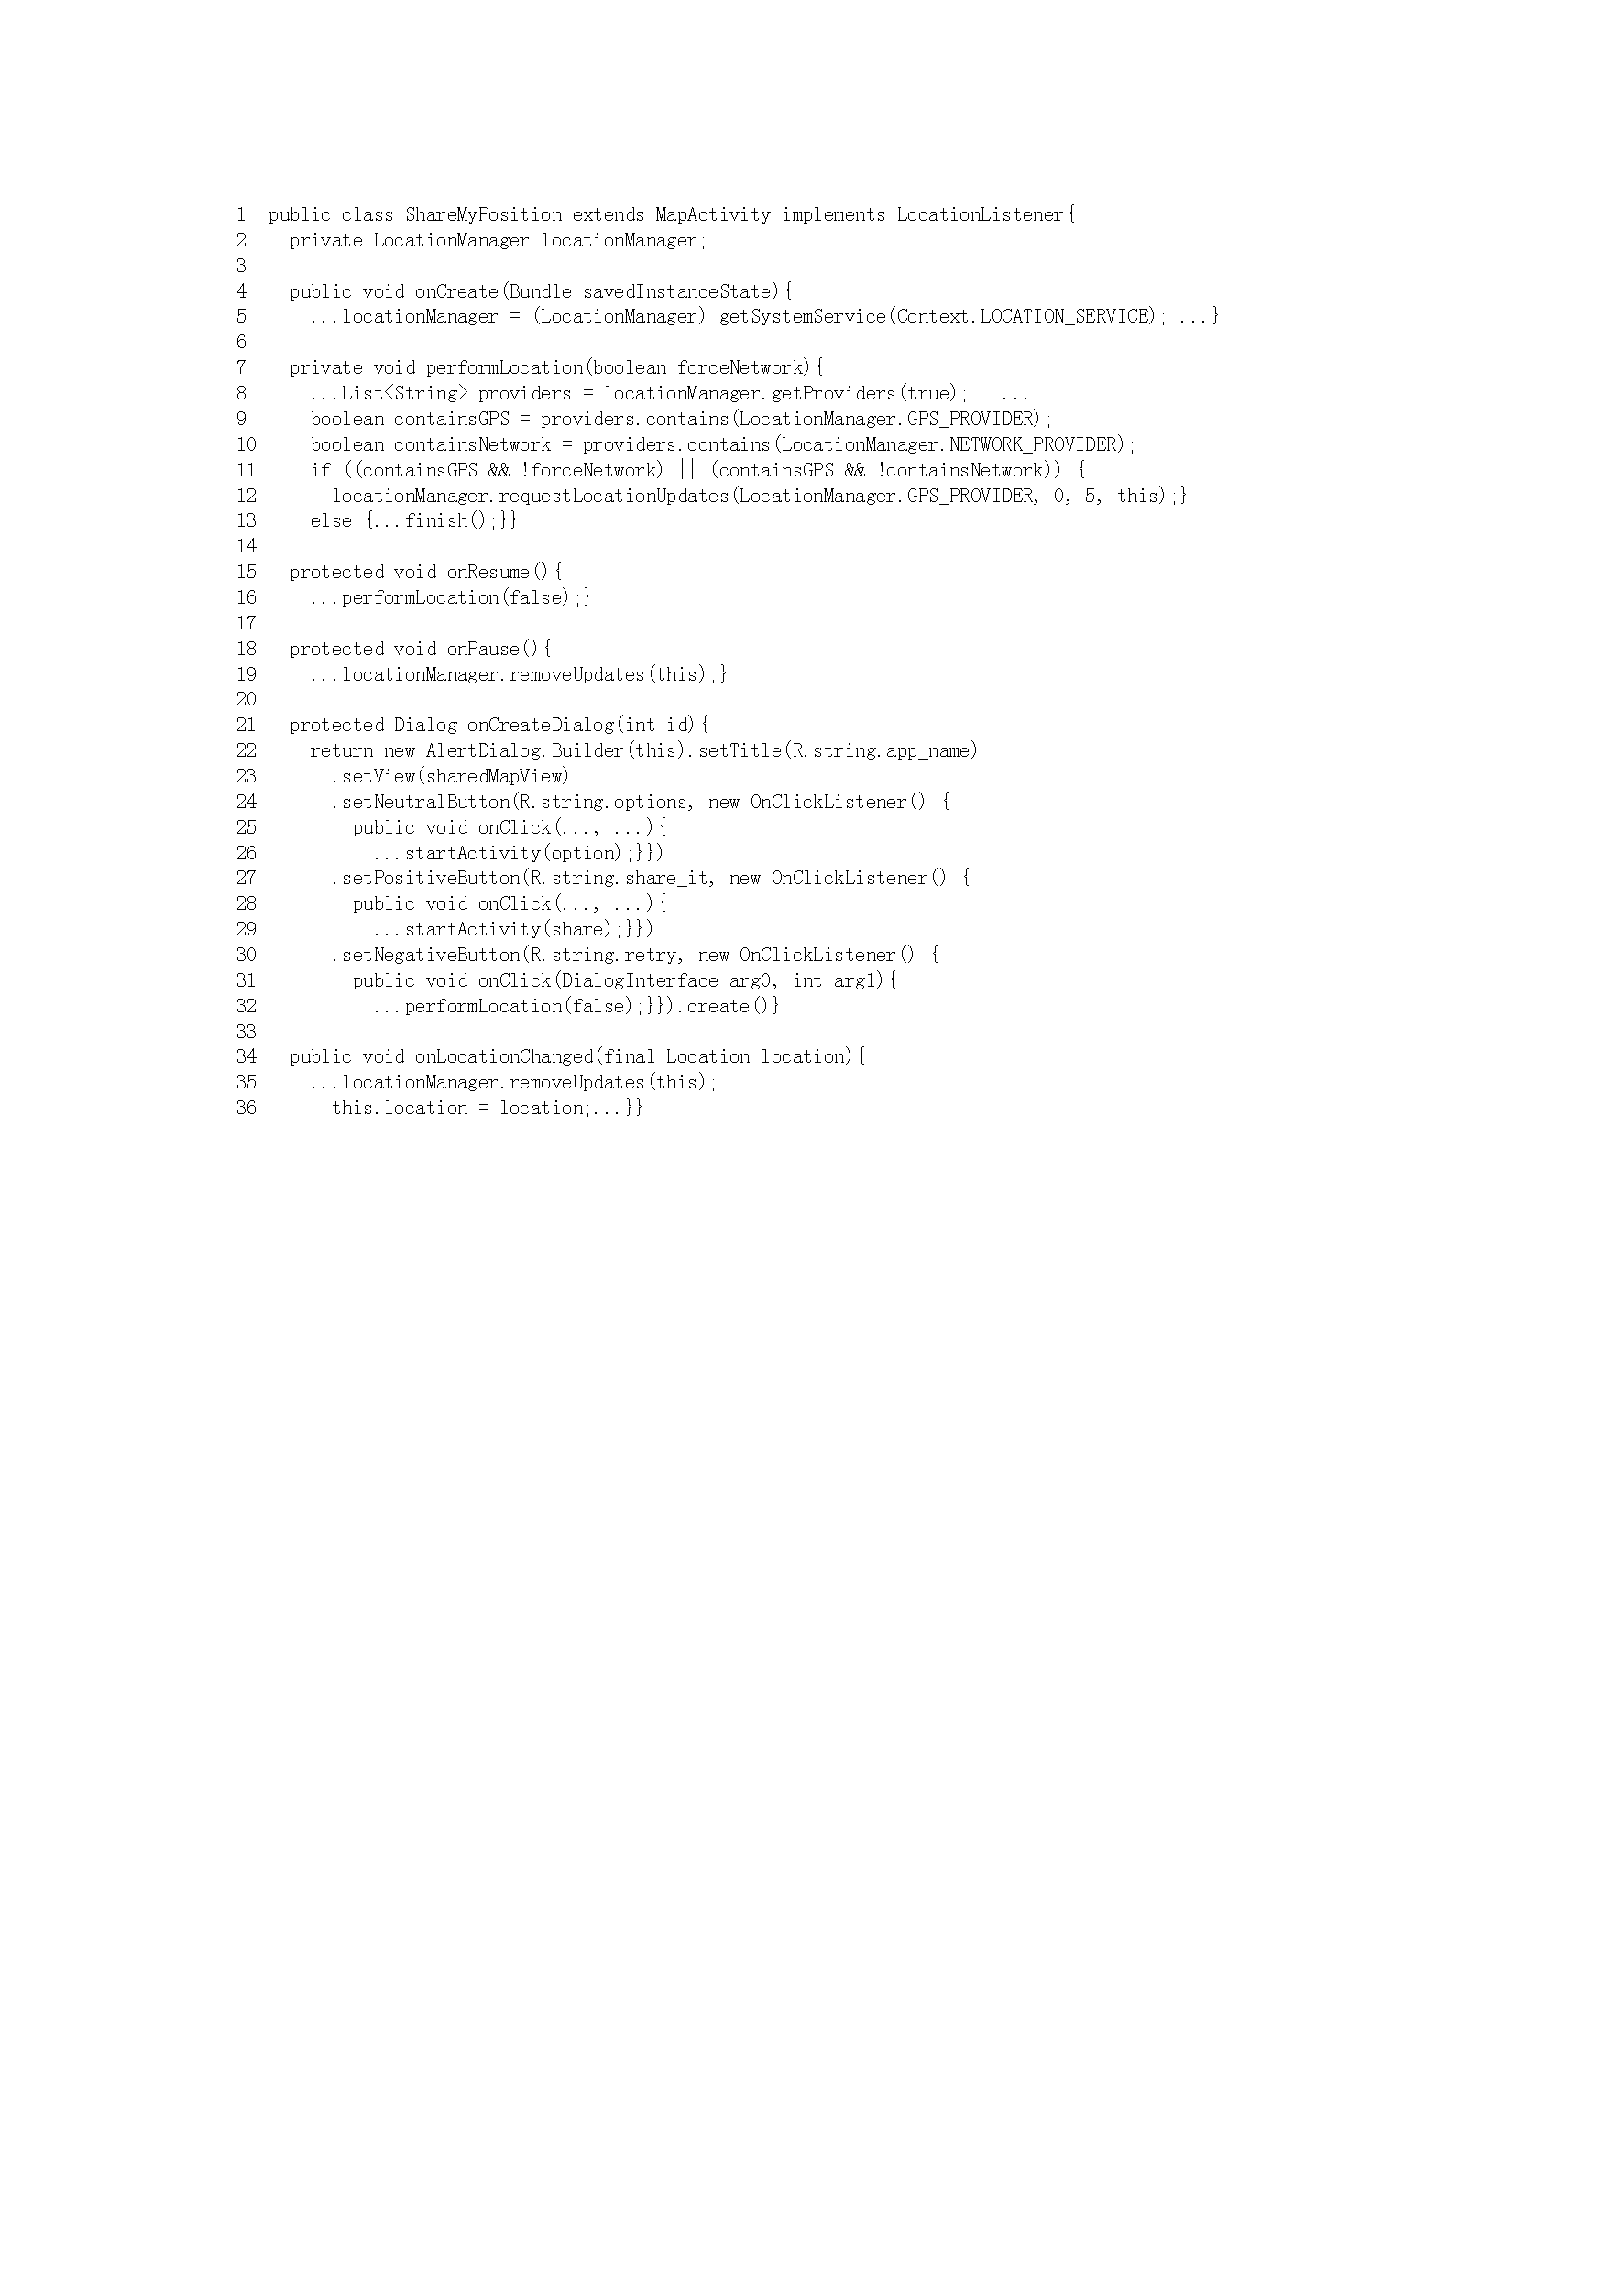
\includegraphics[width=1\linewidth]{pic/motivation1.pdf}  
  \caption{Motivation example derived from ShareMyPosition\cite{newShareMyPosition}.}  
  \label{fig:1}  
\end{figure}

Figure 1 represents partial source code of app \texttt{ShareMyPosition}, which is used to share one's location to others. The main activity \texttt{ShareMyPosition} contains three lifecycle callbacks (\texttt{onCreate} (line 4, 5), \texttt{onResume} (line 15, 16) and \texttt{onPause} (line 18, 19)), as well as a system-driven callback (\texttt{onLocationChanged} (line 34-36). The main activity implements a listener interface \texttt{LocationListener} by overriding its method \texttt{onLocationChanged}. In the \texttt{onCreate} callback, ShareMyPosition defines and assigns a \texttt{LocationManager} variable \texttt{locationManager}. Then in the \texttt{onResume}, the \texttt{locationManager} variable is used to register the callback listener \texttt{this} via a self-defined method \texttt{performLocation}. 
Rather than registering it directly, the \texttt{performLocation} first judges whether one of the conditions \texttt{containsGPS \&\& !forceNetwork} and \texttt{containsGPS \&\& !containsNetwork} is satisfied (line 11). If so, the \texttt{this} object is registered as listener; otherwise, the lifecycle finishes. The system-driven callback \texttt{onLocationChanged} is activated along with the register action, but inactivated after the \texttt{this} listener is unregistered in the \texttt{onPause} or \texttt{onLocationChanged} callback. Besides of the system-driven callback, there exists three \textit{GUI} callbacks in function \texttt{onCreateDialog} (line 21-32). These callbacks will be invoked when certain \textit{button-clicked} event fires. Especially the event on \textit{PositiveButton} (line 27-29) and \textit{NeutralButton} (line 24-26) will trigger a new activity.

 
\subsection{Problem Definition}\label{problem-define}
The example in Figure \ref{fig:1} makes traditional \textit{CCFG} (\textit{CCF} graph) construction challenging. First, system-driven callback \texttt{onLocationChanged} is not directly invoked in the holder callback \texttt{onResume}. Instead, whether it is invoked is determined by the calculation of several condition variables (\texttt{containsGPS}, \texttt{forceNetwork}, etc.). One can simply ignore these condition variables and assume that all the invoker can be connected with the invokee callbacks, but this would result in significant confusion in traversing the callback flow model. To this end, a path-insensitive control flow impacts the precision of generated model. 

Second, lifecycle callbacks emerging in the example includes not only \texttt{onCreate}, but also
\texttt{onResume} and \texttt{onPause}. Traditional modelling manners handle the lifecycle callbacks in a coarse-grained way that only start (i.e. \texttt{onCreate}) and end (i.e. \texttt{onDestroy}) nodes are taken into consideration. Although it appears to be easy to handle the sequences of fine-grained callbacks like \texttt{onResume} and \texttt{onPause} among lifecycle callbacks, the modelling faces \textit{jumping confusion} once non-lifecycle callbacks are involved. In our example, the \texttt{onClick} in line 28 takes a connection to start the activity \texttt{share} which can be denoted as \texttt{PositiveButton.onClick} $\rightarrow$ \texttt{share.onCreate}. In theory, the \texttt{onPause} is known to be invoked when current activity loses its focus, so that it should be invoked before \texttt{share.onCreate}. Thus the path \texttt{PositiveButton.onClick} $\rightarrow$ \texttt{ShareMyPosition.onPause} $\rightarrow$ \texttt{share.onCreate} is supposed to be created. However, the \texttt{ShareMyPosition.onPause} $\rightarrow$ \texttt{share.onCreate} becomes invalid when other paths pass. A typical invalid path is \texttt{NeutralButton.onClick} $\rightarrow$ \texttt{ShareMyPosition.onPause} $\rightarrow$ \texttt{share.onCreate}. Cases as the example make jumping action between activities confused. Apart from jumping confusion, the fine-grained hybrid model would result in other unexpected conflicts between lifecycle and non-lifecycle callbacks. Assuming that an \texttt{onClick} callback is registered in the \texttt{onCreate}, there should be an edge connecting the two callbacks. However, this edge would become invalid when encountering \texttt{onResume}, since the \texttt{onResume} should always be first invoked after the \texttt{onCreate}.

Another challenge in the \textit{CCFG} construction is the representation of inter-components, which is not explicit presented in the motivation example. As mentioned in Section \ref{background}, the objective component in the inter-components jumping can be either service or activity. The jumping for activity can be treated as normal control flow since the invoker and invokee occur one after another. For the service, however, the jumping just acts as a launcher for triggering the objective component. There is not a strict time sequence between invoker and invokee in service case, because service runs in a parallel way with other components. A fine-grained modelling has to distinguish the two types of jumping.

%Apart from activity, other three domain components: service, broadcastReceiver and content provider also play important roles in constructing general callback model. Similar with the jumping between activities, the transition between different components types is also under a certain container callback within the previous component. However, the program of different components can be executed in a parallel way. For example, a service is able to running in background at the time a foreground activity in the same app is active. Thus the traditional control flow graph is hard to represent the program logic between components of different types. Especially, component like service has its own lifecycle as activity does. Completely considering every status appears quite challenging. To this end, we propose a novel representation to describe the generic model, especially for the model across components, within an app. We introduce this representation in section \ref{transition-model}.

%\textbf{Path-sensitive}. Considering \textit{path-sensitive} within target program benefits a lot for the precision of control flow analysis\cite{}. Traditional callback models \cite{} are seldom considering path-sensitive, leading to the generated model just works as a architecture reflection for aided analysis. That is to say, a path-insensitive model could not directly be used for applied testing, verification or security analysis, causing these techniques need more flow details guiding the execution. In our example, whether the \texttt{onLocationChanged} is active or not is dependent on the predicates at conditional branch instructions. If the modelling discards considering the branch predicates, it is impossible to distinct whether the callback fires in an absolute way under its container callback(\texttt{onResume} in this case) or not. Such details could directly impact processing of high-level techniques upon the generated model, such as generation of test case (for testing) and logic properties (for model verification and security analysis).

%We address the path-sensitive challenges using data dependency analyses introduced in section \ref{path-sensitive}. 
  
%\textbf{Fine-grained lifecycle}
%Handling fine-grained lifecycles like \texttt{onResume} and   \texttt{onPause} is of importance for constructing a complete callback model. For the processing of system listener register, the register and unregistered sentences are often located in \texttt{onResume} and \texttt{onPause} callbacks. Therefore, analysis towards these lifecycle callbacks is indispensable.

%Usually, these sorts of callbacks are designed to be invoked in some specific time according to the activity's running status, e.g., losing focus or recovering focus. Each time when current activity jump to a new one, the fine-grain lifecycle like \texttt{onPause} and \texttt{onStop} will be invoked in sequences. Since the destinations of activity jumping may be different (e.g., the \texttt{share} and \texttt{option}), it has to generate two different paths for the two jumping. However, both of the two paths contain the same fine-grained lifecycle callbacks. One simple tackling manner is to generate a copy fine-grain lifecycle for each path, but it can yield redundancy nodes and edges, which will impact the traverse cost and model precision. So how to generate a reasonable model which can properly handle the fine-grain lifecycle callbacks becomes a challenge. We propose our solution in section \ref{fine-grain lifecycle}.